\documentclass[aps,prl,twocolumn,nofootinbib,showkeys, nolongbibliography, 10pt]{revtex4-2} 


\synctex=1 

%========================= PACKAGES ==================================
\usepackage{dcolumn}
\usepackage{color}
\usepackage{makecell}
\usepackage{tabularx, graphicx}
\usepackage{latexsym}
\usepackage{colortbl}
\usepackage{psfrag}
\usepackage{bbm,bm,array,physics}
\usepackage{dsfont}
\usepackage{float, mathrsfs}

\usepackage{amsmath,amssymb} 
\usepackage{graphicx,comment}

\usepackage[tight]{subfigure} 

\usepackage[dvipsnames]{xcolor} 
\usepackage[papersize={8.5in,11in}]{geometry}
\usepackage[colorlinks=true]{hyperref}
\hypersetup{
    bookmarks=true,         % show bookmarks bar?
    unicode=false,          % non-Latin characters 
    pdftoolbar=true,        % show Acrobat
    pdfmenubar=true,        % show Acrobat 
    pdffitwindow=false,     % window fit to page when opened
    pdfstartview={FitH},    % fits the width of the page to the window
    pdfkeywords={keyword1} {key2} {key3}, % list of keywords
    pdfnewwindow=true,      % links in new window
    colorlinks=true,       % false: boxed links; true: colored links
    linkcolor=magenta, %red,          % color of internal links (change box color with linkbordercolor)
    citecolor=blue,        % color of links to bibliography
    filecolor=magenta,      % color of file links
    urlcolor=blue           % color of external links
} 

\geometry{top=1.5cm, left= 1.5 cm, right= 1.5 cm, bottom= 1.5 cm}        





\def \nn{\nonumber \\}
\def\*#1{\mathbf{#1}} %\bold font
\newcommand{\at}[2][]{#1|_{#2}}


%=======================================================================
\begin{document}
\title{Deriving Fermi arcs of generic nature spanning nodes featuring multibands, nonlinear dispersion, and/or multipoles}


\author{Ipsita Mandal}


\affiliation{Department of Physics, Shiv Nadar Institution of Eminence (SNIoE), Gautam Buddha Nagar, Uttar Pradesh 201314, India}




\begin{abstract}
%%%%%%%%%%%%%%%%%%%%%
Fermi arcs appear as the surface states at the boundary of a three-dimensional topological semimetal with the vacuum, reflecting the Chern number ($\mathcal C$) of a nodal point in the momentum space, which represents singularities (in the form of monopoles) of the Berry curvature. They are finite arcs, attaching/reattaching with the bulk-energy states at the tangents of the projections of the Fermi surfaces of the bands meeting at the nodes. The number of Fermi arcs emanating from the outermost projection equals $\mathcal C$, revealing the intrinsic topology of the underlying bandstructure, which can be visualised in experiments like ARPES. Here we outline a generic procedure to compute these states for generic nodal points, (1) whose degeneracy might be twofold or multifold; and (2) the associated bands might exhibit isotropic or anisotropic, linear- or nonlinear-in-momentum dispersion. This also allows us to determine whether we should get any Fermi arcs at all for $\mathcal C = 0$, when the nodes host ideal dipoles.
%%%%%%%%%%%%%%%%%%%%%%%%%%%%%%%%%%%%%%
\end{abstract}

\keywords{Berry curvature, Fermi arcs, Surface states, Topology} 

\maketitle



%=========================  =========================
%{\it Introduction.---} 
Nodal points (NPs) in three-dimensional (3d) semimetals represent defective points in the Brillouin zone (BZ), where $(2\, \varsigma + 1)$ bands cross at a nodal-point degeneracy [see Fig.~\ref{figdis}(a)]. In the vicinity of a nodal point, the bands form a spin-$\varsigma$ representation of the SU(2) group. They provide an intriguing crucible to observe mathematical notions of topology playing out in real-life systems~\cite{burkov11_Weyl,hosur1, armitage_review, hosur-review, yan17_topological, ips-kush-review, bernevig, bernevig2, grushin-multifold, claudia-multifold} because they are the singular points of the Berry-curvature (BC) where it blows up, hosting a BC-monopole synonymous with the net Chern number ($\mathcal C $) at the NP.
%%%%%%%%%%%%%%%%%%%%%%%%%%%%%%
An isotropic Weyl node, appearing in Weyl semimetals (WSMs)~\cite{burkov11_Weyl, armitage_review, yan17_topological}, carrying $\varsigma = 1/2$, is the poster child of such systems, depicting the simplest scenario. The ubiquitousness of the NPs is reflected by WSMs' multifold cousins like the triple-point semimetals (with $\varsigma = 1 $) and Rarita-Schwinger-Weyl (RSW) nodes (with $\varsigma = 3/2$)~\cite{bernevig, long, isobe-fu, tang2017_multiple, ma2021_observation, prb108035428, grushin-multifold, ips-rsw-ph, ips-shreya,ips-exact-rsw}. The singularity of the BC at an NP \cite{xiao_review, sundaram99_wavepacket, graf-Nband} goes beyond the monopole-character, as the possibility of ideal BC-dipoles and higher-order poles have been predicted \cite{twoband-dipole, graf-hopf, hopf2, hopf3}, when considering a multipole expansion of the Berry connection [cf. Fig.~\ref{figdis}(b)].


%%%%%%%%%%%%% fig 0 %%%%%%%%%%%%%%%%%%%%%
\begin{figure*}[t]
\centering
\subfigure[]{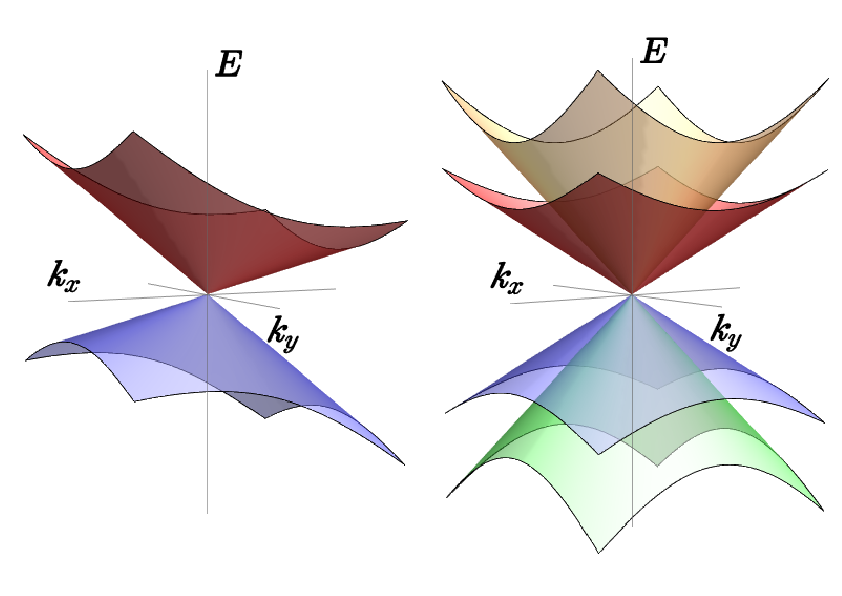
\includegraphics[width=0.35\textwidth]{disp-prl}}\hspace{ 2 cm }
\subfigure[]{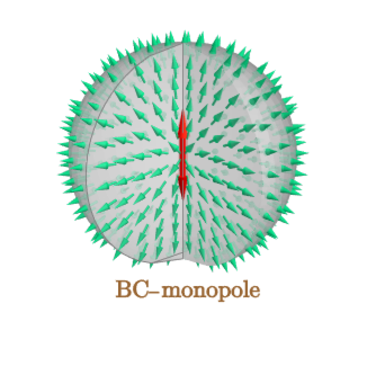
\includegraphics[width=0.27 \textwidth]{mono-apl}\hspace{-1 cm}
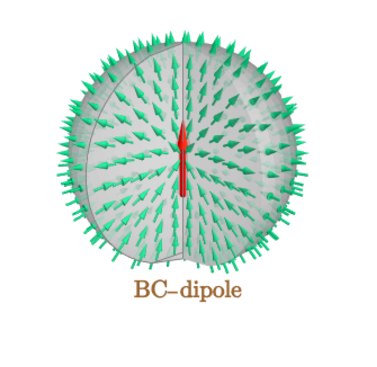
\includegraphics[width=0.27 \textwidth]{dipole-apl}}
\caption{(a) Dispersion ($E$) of the bands, crossing at a tilted Weyl node and a fourfold-degenerate Rarita-Schwinger-Weyl node, against the $k_x k_y$-plane. (b) Schematics of BC-flux field in the 3d momentum space for a monopole and an ideal dipole.
\label{figdis}}
\end{figure*}
%%%%%%%%%%%%%%%%%%%%%%

Often our study of the intrinsic topology of the 3d BZ, when treated as a 3d manifold, involves identifying unambigous quantitative signatures of the topological invariants like $\mathcal{C}$. Arguably Fermi arcs provide the most undisputed observables \cite{yang_Weyl, lv_Weyl_arc, sanchez, spin1-arc,shroter-arc, Yao2020, multifold-rhsi-arc, quad-weyl-arc}, as contemporary experiments like angle-resolved photoemission spectroscopy (ARPES) can clearly visualise them. Physically, they emerge as the loci of the edge-states of 2d slices of the 3d BZ, when we take a surface (say, whose outward normal is along the unit vector, $\boldsymbol{\hat n}$) of a slab of a  topological semimetal. In fact, these surface states arise due to the presence of chiral edge modes of the 2d slices, after we impose open boundary conditions on those slices \cite{burkov11_Weyl, hosur1, hosur-review}. Although we can no longer describe the system in the momentum space for the direction along $\boldsymbol{\hat n}$, the momentum-components perpendicular-to-$\boldsymbol{\hat n}$ (say, $\mathbf k_\parallel$), i.e. parallel to the surface itself, remain good quantum numbers (as long as we consider very large spatial dimensions along those directions). Thus, a single surface (or boundary) in real space gives us a surface Brillouin zone (SBZ), spanned by the components of $\mathbf k_\parallel$, and hosting the Fermi arcs. Although the analytical derivation of surface states, which take the form of Fermi arcs in NPs, is well-understood for WSMs \cite{witten, hashimoto-arc-weyl, babak-arc-weyl, inti-arc-weyl}, for most other cases, the derivations are system-specific and not generic-enough \cite{witten, okugawa-arc-weyl, liu-arc-mutiweyl, jafari-arc-weyl, trauzettel-arc-weyl, ewelina-surface-states} to be applicable for arbitrary cases of dispersion (for example, anisotropic and/or nonlinear-in-momentum behaviour) and band-crossings. In this Letter, our aim is to outline a generic procedure to obtain the analytical forms of the Fermi arcs and demonstrate its effectiveness by applying it to a variety of NPs.



%%%%%%%%%%%%%%%%%%%%%%%%%%%%%%%%%%%%%%%%%%%

Let us take a single surface at $x=0$ such that the $x<0$ region represents a semi-infinite semimetal, with the bulk Hamiltonian $H(\mathbf k)$, where $\mathbf k \equiv \lbrace k_x, k_y, k_z \rbrace $ and $k =\sqrt{k_x^2 + k_y^2 + k_z^2}$. The translation symmetry is broken along the $x$-axis, and we use the Hamiltonian,
$ H_x = H (k_x \rightarrow -i \, \partial_x , k_y, k_z)$. Demanding that $H_x $ be Hermitian in the region $x \in [0, \infty)$, we have the physical condition that
\begin{align}
\label{eqherm}
 \int_0^\infty  dx \,\psi^\dagger (x) \, H_x\,\phi (x) = 
 \int_0^\infty  dx\, [H_x\, \psi(x) ]^\dagger\,\phi(x) \,,
\end{align}
%%%%%%%%%%%%%%%%
while considering two bonafide boundary-states, $\psi $ and $\phi$. The current-density operator is defined as
$ j_x \equiv \partial_{k_x}  H(\mathbf k) \vert_{k_x \rightarrow -i\, \partial_x}$.
%%%%%%%%%%%%%%%%
Consequently, Eq.~\eqref{eqherm} also translates into a physically-sensible boundary condition (bc) which prohibits the current transmission through the boundary via $ (\psi^\dagger \, j_x \, \psi )\vert_{x=0}= 0$, alternatively known as the hard-wall bc. The boundary modes must behave as decaying wavefunctions of the form of $
\psi (x) = \psi_0 \, e^{- \kappa \, x}$, with $ \text{Re}(\kappa) > 0$, so that the surface states are bound to the boundary at $ x= 0 $. Here, $\psi_0$ is independent of $x$ and any $x$-dependence of $\psi(x)$ is assumed to be contained in the $ e^{- \kappa \, x}$ factor. 


The effective Hamiltonian in the vicinity of a single Weyl node [cf. Fig.~\ref{figdis}(a)] is captured by
\begin{align}
\label{eqweyl}
H_W (\mathbf k) = \boldsymbol{\sigma} \cdot {\mathbf k}\,,
\end{align}
for which Eq.~\eqref{eqherm} translates into
$\psi^\dagger (x)\, \sigma_x \, \phi (x) \vert_{x=0} = 0
\Rightarrow j_x\vert_{x=0} \equiv \psi_0^\dagger\, \sigma_x \, \phi_0  = 0$.
%%%%%%%%%%%%%%%%%%%%%%%%%%%
Witten \cite{witten} prescribed an energy-independent boundary condition,
\begin{align}
\label{eqalpha}
\Psi_0 =  M \, \Psi_0\,, \text{ where } M = \cos \alpha \, \sigma_y + \sin  \alpha \, \sigma_z \,,
\end{align}
%%%%%%%%%%%%
as a local linear restriction on the components of the spinor wavefunction.
This is a good boundary condition because $\sigma_x $ anticommutes with $M$, leading to
$
 \psi_0^\dagger\, \sigma_x \, \phi_0 = 
 \frac{1}{2} \left[ \psi_0^\dagger\, \sigma_x \,M\, \phi_0 
 + ( M\, \psi_0)^\dagger\, \sigma_x \, \phi_0 \right ]  = 0$.



%%%%%%%%%%%%% fig 1 %%%%%%%%%%%%%%%%%%%%%
\begin{figure*}[t]
\centering
\subfigure[]{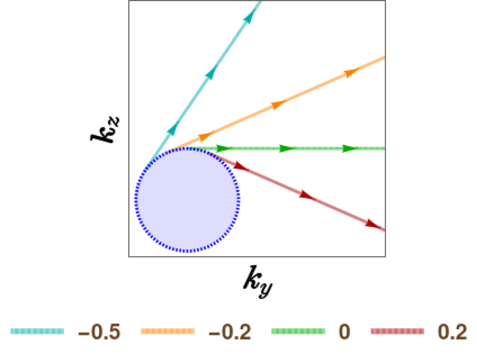
\includegraphics[width=0.27 \textwidth]{weyl}} \hspace{ 2 cm}
\subfigure[]{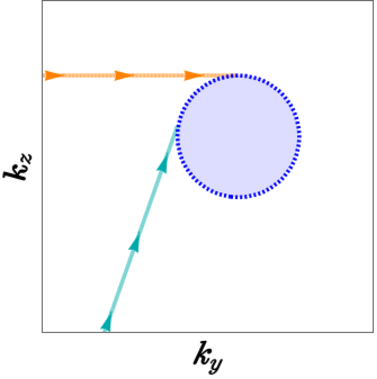
\includegraphics[width=0.2\textwidth]{tsm}} \hspace{ 2 cm}
\subfigure[]{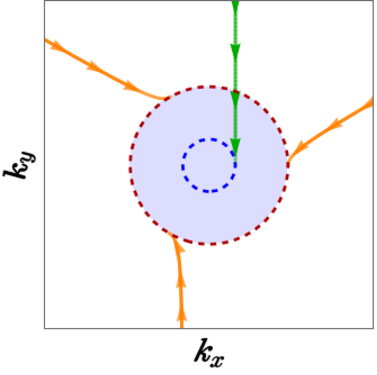
\includegraphics[width=0.2\textwidth]{rsw}}
\caption{(a) Tilted Weyl node with $\eta =0.35 $: Each Fermi arc corresponds to a distinct value of $b_1$, colour-coded as shown in the plot-legends. (b) TSM node: 2 Fermi arcs entering into FS-projection. (c) RSW node: 4 Fermi arcs entering into the FS-projections. The dashed circles represent the projections of the bulk FSs with $\mu =0.5$.
\label{fig_weyl}}
\end{figure*}
%%%%%%%%%%%%%%%%%%%%%%



For generic nodes with multifold bands and/or nonlinear powers of the components of $\mathbf k$, Witten's trick will not work, which we will explicitly see why considering some specific examples. Hence, we need an unambigous generic method applicable to derive the equations describing the curves representing the relevant Fermi arcs, which we elucidate here. Suppose we have an $N$-fold degeneracy at a node, described by the $N \times N $ Hamiltonian, $H_N (\mathbf k)$, in the bulk BZ. Let us look for surface states where the surface-normal is along the direction denoted by the unit vector, $\boldsymbol{\hat n}$, and located at $r_\perp = 0$, where $ r_\perp \equiv \mathbf r \cdot \boldsymbol{\hat n}$. We set our convention that the region $ r_\perp <0 $ represents the region occupied by the semimetallic material, while $r_\perp >0 $ represents the adjoining non-topological region (e.g., vacuum). Dividing up the momentum components along and perpendicular to $\boldsymbol{\hat n}$ as $  k_\perp$ and $\mathbf k_\parallel $, respectively, the boundary Hamiltonian is obtained as
$ H_{r_\perp} = H_N ( k_\perp\rightarrow -i \, \partial_{r_\perp} , \mathbf k_\parallel)$.
The imposition of the Hermiticity condition on $H_{r_\perp}$ leads to
\begin{align}
\label{eqherm1}
 \int_0^\infty  dr_\perp \,\psi^\dagger (r_\perp) \, H_{r_\perp}\,\phi (r_\perp) = 
 \int_0^\infty  dr_\perp\, [ H_{r_\perp}\, \psi(r_\perp) ]^\dagger\,\phi(r_\perp) \,,
\end{align}
analogous to Eq.~\eqref{eqherm}. Let us parametrise a solution as
\begin{align}
& \psi (r_\perp) = \psi_0 \, e^{- \kappa \, r_\perp} ,
\text{ with } \text{Re}(\kappa) > 0
\text{ and} \nn
& \psi_0^T  = \begin{bmatrix}
1 & a_1 +i \, b_1 & a_2 + i \, b_2 & \cdots & a_{N-1} + i \, b_{N-1}
\end{bmatrix}.
\end{align}
As argued earlier, will turn out to be equivalent to the condition of
%%%%%%%%
\begin{align}
\label{eqcur}
&\psi^\dagger  (r_\perp)\, j_{r_\perp} \psi (r_\perp) \big \vert_{r_\perp=0}= 0\,,
 \text{ where} \nn &
 j_{r_\perp} \equiv \partial_{k_\perp}  H_N(k_\perp,  {\mathbf k_\parallel} ) 
\big \vert_{k_\perp \rightarrow -i\, \partial_{r_\perp} }
\end{align}
represents the current-density operator perpendicular to the surface. Next, we need to solve for the eigenvalue equation,
\begin{align}
\label{eqhambdy}
H_{r_\perp} \psi (r_\perp) = E\, \psi (r_\perp)\,,
\end{align}
%%%%%%%%%%%%%%%%%
which leads to $N$ complex-valued equations involving the $(2N+1)$ unknown variables, $ E$,
$\kappa_r \equiv \text{Re}(\kappa)$, $\kappa_i \equiv \text{Im}(\kappa)$, $a_1$, $ b_1$, $a_2$, $ b_2$, $\cdots$, $a_{N-1}$,
and $b_{N-1}$. This implies that we have $(2N+1)$ real equations [on including the real equation coming from Eq.~\eqref{eqcur}] at our disposal, which we can use to solve for the same number of unknown variables. In the next section, we will study a variety of systems to see that the above procedure works generically.



Let us consider the one-node model given by Eq.~\eqref{eqweyl}, where we want to consider a boundary at $x=0$, indicating $\boldsymbol{\hat n} = \boldsymbol{\hat x} $. Using $ \psi_0^T  = \begin{bmatrix}
1 & a_1 +i \, b_1 \end{bmatrix}$, we get $E = \frac{2 \,b_1\, k_y +(1- b_1^2)\, k_z} { 1 + b_1^2 }$, $\kappa_r = \frac{\left(b_1^2-1\right) k_y+2 \,b_1\, k_z} { 1 + b_1^2 } $, and $\kappa_i = 0$.
%%%%%%%%%%%%%%%%%%%%%%%%%%%%%%%
%{\it Tilted Weyl nodes.---} 
The bulk Hamiltonian in the vicinity of a node, tilted with respect to the $k_x$-axis, is captured by $ H_W (\mathbf k) = \boldsymbol{\sigma} \cdot {\mathbf k} + \eta\, k_x \, {\mathbb{I}}_{2\times 2}$.
For this case, on using $ \psi_0^T  = \begin{bmatrix}
1 & a_1 +i \, b_1 \end{bmatrix}$, we obtain the solutions as $E =  \frac{b_1 \left [\sqrt{1-\left( 1 + b_1^2 \right)\,
 \eta ^2}+1\right ] k_y+  \left[ \sqrt{1-\left( 1+ b_1^2 \right)\, \eta ^2}  - b_1^2 \right]
 k_z } { 1 + b_1^2} $, 
$\kappa_r  = \frac{\left(b_1^2-1\right) k_y+2 \,b_1\, k_z} { 1 + b_1^2} $, $\kappa_i = 0$, and $a_1 =
\frac{\sqrt{1-\left( 1 + b_1^2\right) \eta ^2} \, -1} {\eta }$.
%%%%%%%%%%%%%%
Fig.~\ref{fig_weyl}(a) illustrates the Fermi arcs for four distinct values of $b_1$, with $\eta$ set to $0.35$. Each arc grazes onto the projection of a Fermi surface (FS).
 
 


Let us now consider bands carrying pseudospin-1 quantum numbers crossing at threefold-degenerate nodes \cite{bernevig, spin13d1, ips-magnus, grushin-multifold, ips-spin1-ph, ips-exact-spin1, ips-internode}, representing the so-called triple-point semimetals (TSMs). These are three-band generalisations of the pseudospin-1/2 quasiparticles in Weyl semimetals, with the nodal points acting as Berry-curvature monopoles of magnitude 2. The effective low-energy continuum Hamiltonian, in the vicinity of a threefold nodal point, is given by
$\mathcal{H}_{T}(\mathbf  k) = {\mathbf k} \cdot \boldsymbol{\mathcal S}$, where $ \boldsymbol{\mathcal S} $ represents the vector spin-1 operator with three components \cite{ips-spin1-ph, ips-exact-spin1, ips-internode}.
%%%%%%%%%%%%%%%%%%%%%%
Here we note that, although this is a straightforward generalisation of the isotropic Weyl node, we cannot apply Witten's method simply because of the fact that $ \mathcal S_x$, $\mathcal S_y$, and $ \mathcal S_z $ \textit{do not anticommute} (unlike the Pauli matrices). We use the parametrisation $ \psi_0^T  = \begin{bmatrix}
1 & a_1 +i \, b_1 & a_2 + i\, b_2 \end{bmatrix}$ and consider a boundary at $x=0$. Plugging it in Eqs.~\eqref{eqcur} and Eq.~\eqref{eqhambdy}, the solutions indeed tell us that there are two Fermi arcs characterised by (1) $E =\frac{2 \sqrt{2}\, b_1\, k_y+4 \,k_z}{ 2 + b_1^2 }-k_z$, $ \kappa_r = \frac{\left(b_1^2-2\right) k_y+2 \sqrt{2} \,b_1\, k_z} { 2 + b_1^2} $, $\kappa_i=0$, $a_1 = 0$, $a_2 = -\, b_1^2/2$, $|b_1 | > 0$, and $b_2 =0$; and (2)  $E = k_z$, $ \kappa_r = -\, k_y $, $\kappa_i=0$, $a_1 = 0$, $a_2 = 0$, $ b_1 = 0$, and $b_2 =0$.
%%%%%%
Fig.~\ref{fig_weyl}(b) illustrates the Fermi arcs for $\mu=0.5$ and $b_1=-1$. Since $ |\mathcal C| = 2$, we observe two arcs entering into the FS-projection.

%%%%%%%%%%%%% fig 2 %%%%%%%%%%%%%%%%%%%%%
\begin{figure*}[t]
\centering
\subfigure[]{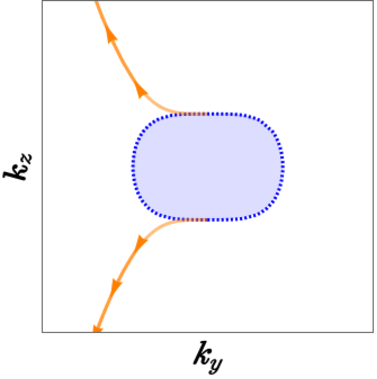
\includegraphics[width=0.2 \textwidth]{double-weyl}} \hspace{ 0.5 cm}
\subfigure[]{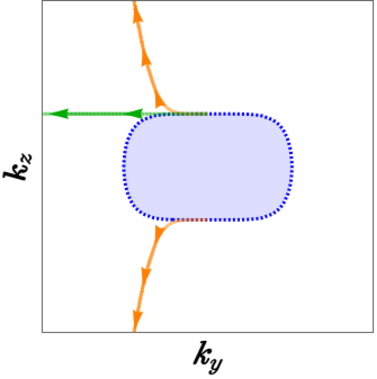
\includegraphics[width=0.2\textwidth]{triple-weyl}} \hspace{ 0.5 cm}
\subfigure[]{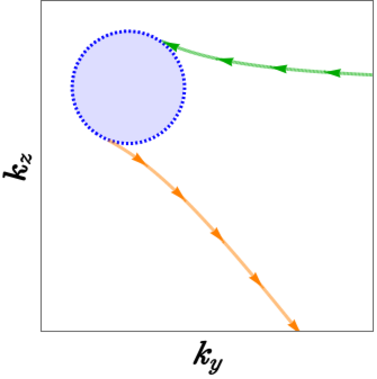
\includegraphics[width=0.2\textwidth]{dipole1}} \hspace{ 0.5 cm}
\subfigure[]{\includegraphics[width=0.155 \textwidth]{dipole2}}
\caption{(a) Double-Weyl node: 2 Fermi arcs leaving from the FS-projection. (b) Triple-Weyl node: 3 Fermi arcs leaving from the FS-projection. (c) and (d) represent the models with BC-dipole with two and three bands, respectively. In subfigure (d), arcs for 4 distinct values of $b_1$ have been shown.
\label{figdipole}}
\end{figure*}
%%%%%%%%%%%%%%%%%%%%%%



Next we focus on bands carrying pseudospin-3/2 quantum numbers crossing at fourfold-degenerate NPs [cf. Fig.~\ref{figdipole}(a)], widely known as the RSW nodes. They appear at the $\Gamma$-points of chiral crystals with appreciable SOC couplings \cite{grushin-multifold, multifold-rhsi, Yao2020, ips-rsw-ph,*ips-shreya,*ips-internode}, hosting a net BC-monopole of magnitude 4. The effective Hamiltonian, in the vicinity of an isotropic RSW node, takes the form of
%%%%%%%%%%%%%%%%%%%%%%%%%%%%%%%
$
\mathcal{H}(\boldsymbol{k}) =   {\mathbf k} \cdot \boldsymbol{\mathcal J} $,
where $ \boldsymbol{\mathcal J } = \lbrace {\mathcal J }_x,\, {\mathcal J }_y,\, {\mathcal J }_z \rbrace $ represents the vector operator whose three components comprise the angular-momentum operators in the spin-$3/2$ representation of the SU(2) group. Just for the ease of calculations, we consider a boundary at $z=0$ (just because the $\mathcal J$ matrix has fewer nonzero entries, leading to less cumbersome equations to be solved).
Here again we note that, although this is a fourfold generalisation of the isotropic Weyl node, we cannot apply Witten's method since $ \mathcal J_x$, $\mathcal J_y$, and $ \mathcal J_z $ \textit{do not anticommute}. We use the parametrisation $ \psi_0^T  = \begin{bmatrix}
1 & a_1 +i \, b_1 & a_2 + i\, b_2 & a_3 + i\, b_3  \end{bmatrix}$ because of the fourfold nature of the bands. Plugging it in Eqs.~\eqref{eqcur} and Eq.~\eqref{eqhambdy} yield the explicit solutions which are long and cumbersome. In Fig.~\ref{fig_weyl}(c), we pictorially show them for a specific case.




Double-Weyl nodes can be found in materials like $\mathrm{HgCr_2Se_4}$~\cite{Gang2011} and $\mathrm{SrSi_2}$~\cite{hasan_mweyl16, singh18_tunable}, which exhibit a hybrid of linear dispersion (chosen to be along the $k_z$-axis) and quadratic dispersion (in the $k_x k_y$-plane). In the vicinity of such a nodal point, the low-energy effective continuum Hamiltonian is given by \cite{bernevig,bernevig2, fu22_thermoelectric, ips_rahul_ph_strain, ips-ruiz, ips-tilted, chen16_thermoelectric}
$ H_{dW} = \boldsymbol{d} \cdot \boldsymbol{\sigma}$, where
$  \boldsymbol{d} \equiv \left\{ d_x,\, d_y, \, d_z \right\} = \left\{
k_x^2-k_y^2, \, 2 \,k_x \,k_y,\, k_z\right\} $.
%%%%%%%%%%%%
Plugging in the parametrisation of $ \psi_0^T  = \begin{bmatrix}
1 & a_1 +i \, b_1 \end{bmatrix}$ in Eqs.~\eqref{eqcur} and Eq.~\eqref{eqhambdy} leads to:
$E = \frac{\sqrt{k_z^2 \cos^2  t-4 \,k_y^4 \tan ^2 t }}
{\cos t}$, $ \kappa _r =  \frac{ s \, k_y}{\cos (t)} $, , where
$a = s \, \frac{ k_z \,\cos t-\sqrt{k_z^2 \cos ^2 t-4 \,k_y^4 \tan^2 t} }
{2\, k_y^2 \left( 1 + \frac{1}{\cos t} \right)}$ and $s = \pm 1$, where $ a_1 = a \cos t$ and $ b_1 = a \sin t$.
Fig.~\ref{figdipole}(a) illustrates the Fermi arcs for $\mu=0.5$ and $ t = \pi/6 $. Since $\mathcal C =  2$, we observe two arcs emanating from the perimeter of the FS-projection.

 
Analogous to the double-Weyl nodes, there exist triple-Weyl nodes (in materials like transition-metal monochalcogenides~\cite{liu2017predicted}) for which $|\mathcal C| = 3$. The triple-Weyl case comprises a hybrid of linear dispersion (chosen to be along the $k_z$-axis) and quadratic dispersion (in the $k_x k_y$-plane). In the vicinity of such a nodal point, the low-energy effective continuum Hamiltonian is given by \cite{bernevig, bernevig2, fu22_thermoelectric, ips_rahul_ph_strain, *rahul-jpcm, ips-ruiz, *ips-tilted}
$H_{tW} = \boldsymbol{d} \cdot \boldsymbol{\sigma}$, where
$  \boldsymbol{d} \equiv \left\{ d_x,\, d_y, \, d_z \right\} =
 \left\{ k_x^3-3 \,k_x\, k_y^2 , \,  3 \,k_x^2 \,k_y-k_y^3  \right\}$. 
%%%%%%%%%%%%
Plugging in the parametrisation of $ \psi_0^T  = \begin{bmatrix}
1 & a_1 +i \, b_1 \end{bmatrix}$ leads to the required equations. Finding exact analytical solutions is cumbersome because of the cubic roots involved. Instead, we parametrise $a_1 = a\cos t$ and $b_1 =\sin t$, and we show below the solutions for $t=0$:
(1) $E = k_z$, $\kappa_r  = \pm \, k_y$, $\kappa_i = 0$, and $a =  0 $;
(2) $ E = \frac{1}{3} \sqrt{9\, k_z^2-\frac{512 \,k_y^6}{3}}$, $\kappa_r = s \,k_y$, $\kappa^2 = 
\tilde s \,\frac{2 \, k_y }{ \sqrt 3}$, and $ a =  s\, \tilde s\,
\frac{3 \,\sqrt{3} \,k_z-\sqrt{27\, k_z^2-512\, k_y^6}}{64\, k_y^3}$, where $(s, \tilde s )= \pm 1$.
Fig.~\ref{figdipole}(b) illustrates the 3 Fermi arcs for $\mu=0.5$ and $s = 1$ for the solution detailed above.


%%%%%%%%%%%%% fig quad Weyl  %%%%%%%%%%%%%%%%%%%%%
\begin{figure*}[t!]
\centering
\subfigure[]{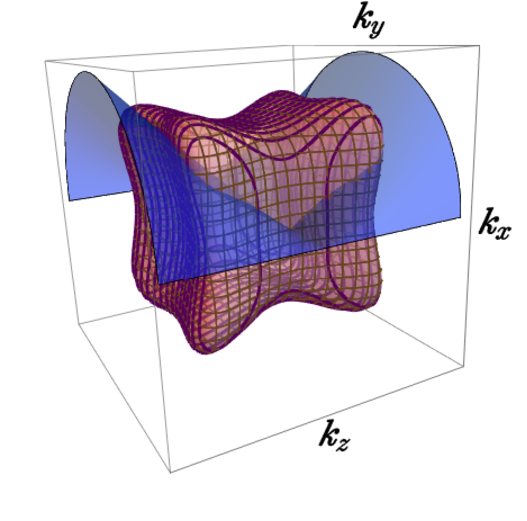
\includegraphics[width=0.22 \textwidth]{qWeyl-prl}}\hspace{ 1 cm}
\subfigure[]{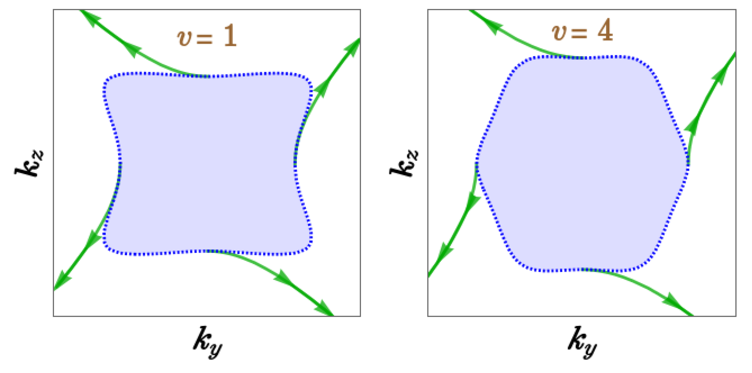
\includegraphics[width=0.4 \textwidth]{qweyl}} 
\caption{(a) The FS-projection is obtained by cutting the 3d FS with the yellow-coloured 2d surface. Here, $\mu=0.25$ and $v = 1$. (b) The Fermi arcs represent modes with $E = 0.25$, emanating from the FS-projection (dashed closed curve) on the $k_y k_z$-plane.
\label{fig_qweyl}}
\end{figure*}
%%%%%%%%%%%%%%%%%%%%%%



In a specific two-band model, the low-energy effective Hamiltonian in the vicinity of a single node harbouring a Berry-dipole [cf. Fig.~\ref{figdis}(b)] is captured by \cite{twoband-dipole}
%%%%%%%%%%%%%%%%%
$ H_{bd} (k_x, k_y, k_z)= 2\, v\, v_z \, k_z \left( k_x \, \sigma_x  +  k_y \,\sigma_y  \right )
+  \left [ v^2 \left( k_x^2 + k_y^2 \right) - k_z^2 \right ] \sigma_z $. 
Since this is a two-band model, we again use $ \psi_0^T  = \begin{bmatrix}
1 & a_1 +i \, b_1 \end{bmatrix}$. We obtain the solutions as $E =  \frac{k_z\, v_z}{b_1^2}
 \left[2 \,b_1 \,v_p \, k_y +\left(b_1^2-1\right) k_z \,v_z\right] $, 
$\kappa_r  =  k_y-\frac{k_z v_z}{b_1 v_p} $, $\kappa_i = 0$, and $a_1= 0 $.
%%%%%%%%%%%%%%
The points on the SBZ where $\kappa_r$ goes to zero are antipodal points, whose tangents are $\propto \pm \lbrace  b_1, -1 \rbrace$. This shows one arc is leaving and another is entering into the bulk states, which are located at the two opposite hemispheres of the FS. These two halves of the FS yield $\pm 1$ on integrating the BC-flux on their surfaces. The helical Fermi arcs reflect the intrinctic dipole-character with $\mathcal C = 0$. Fig.~\ref{figdipole}(c) illustrates the scenario.


  
In Ref.~\cite{graf-hopf}, massless multifold Hopf semimetals have been introduced, which host BC-dipoles at nodes where linearly-dispersing bands cross. We consider the simplest case with a threefold-degenerate node, captured by the effective continuum Hamiltonian \cite{graf-hopf, hopf2, hopf3},
$ H_{H} = k_x \,\lambda_1 + k_y \,\lambda_2+ k_z\,\lambda_5$,
where
$$ \lambda_1 =  \begin{bmatrix}
 0 & 1 & 0 \\
 1 & 0 & 0 \\
 0 & 0 & 0 \\
\end{bmatrix}, \quad
\lambda_2 = \begin{bmatrix}
 0 & -i & 0 \\
 i & 0 & 0 \\
 0 & 0 & 0 \\
\end{bmatrix}, \quad
\lambda_5 = \begin{bmatrix}
 0 & 0 & -i \\
 0 & 0 & 0 \\
 i & 0 & 0 \\
\end{bmatrix} .$$
For this 3-band model, we use the parametrisation $ \psi_0^T  = \begin{bmatrix}
1 & a_1 +i \, b_1 & a_2 + i\, b_2 \end{bmatrix}$. The solutions turn out to be
$E = \frac{ b_1 \,k_y + \sqrt{b_1^2 \left(k_y^2+k_z^2\right)+k_z^2}} { 1 + b_1^2  }$,
$\kappa_r = \frac{ k_z^2 + b_1 \sqrt{b_1^2 \left(k_y^2+k_z^2\right) }-k_y}{ 1 + b_1^2}$, $\kappa_i  = 0 $,
$a_2 = 0 $, and $b_2  =  \frac{\sqrt{b_1^2 \left(k_y^2+k_z^2\right)+k_z^2}\,-b_1 k_y}{k_z}$.
Fig.~\ref{figdipole}(d) demonstrates the nature of the Fermi arcs for some distinct values of $b_1$, which again leads to the picture that one arc is entering and the other leaving the bulk-states. 





A quadruple-Weyl node (QWN) with twofold degeneracy carries $ |\mathcal C| =4 $ \cite{charge4-1, charge4-2, charge4-3, charge4-4} and can exist only in spinless systems at specific time-reversal symmetric points. Thus, they can appear in electronic bandstructures of materials with
negligible SOC-couplings or in the phonon spectra of artificial crystals (such as photonic crystals), all of which can be treated as spinless systems. Let us take the lattice model of Ref.~\cite{charge4-4}, where two nodes of opposite chiralities emerge at the $\Gamma$- and $R$-points. 
For the node sitting at the $\Gamma$-point can be described by the Hamiltonian,
$H_{qW} = \boldsymbol{d} \cdot \boldsymbol{\sigma}$, where
$\boldsymbol{d} \equiv \left\{ d_x,\, d_y, \, d_z \right\}= \left\{\frac{ v \left(k_x^2-k_y^2\right)}{2}, \,\frac{\left(k_x^2+k_y^2-2 \,k_z^2\right)}{2} ,
\,v\, k_x\, k_y\, k_z\right\}$.
%%%%%%%%%%%%
The dispersion is cubic along the $(111)$ direction and quadratic along any other axis. On using $ \psi_0^T  = \begin{bmatrix}
1 & a_1 +i \, b_1 \end{bmatrix}$, the admissible solutions for $\mu \geq 0 $ are: (1) $E = -\, \frac{v \left(k_y^2-k_z^2\right)}
{\sqrt{ 1 + v^2 }}$, $\kappa_r = -\,k_y\, k_z$, $\kappa_i = \pm \, 
\sqrt{\frac{ 2 \,k_z^2 - k_y^2 \left[ v^2 \left(k_z^2-1\right) +1\right ]}
{ 1 + v^2}}$, $a_1= \frac{1}{\sqrt{v^2+1}}$, and $b_1  = \frac{-\, v}{\sqrt{v^2+1}}$; and
(2) $E =  \frac{v \left(k_y^2-k_z^2\right)}{\sqrt{ 1 + v^2 }}$,
$\kappa_r = k_y\, k_z$, $\kappa_i = \pm \, 
\sqrt{\frac{ 2 \,k_z^2 - k_y^2 \left[ v^2 \left(k_z^2-1\right) +1\right ]}
{ 1 + v^2}}$, $a_1= \frac{ -\,1}{\sqrt{v^2+1}}$, and $b_1  = \frac{v}{\sqrt{v^2+1}}$.
%%%%%%%%%%%%%%%%%%%%%%%%%%%%%%%%%%%%%%%%%%%%%%%%%%%%%%%%%%%%%%%%%%%%%
Fig.~\ref{fig_qweyl} illustrates a Fermi surface in the 3d BZ as well as the arcs in the SBZ for $\mu=0.25$, reflecting $\mathcal C = 4$.


%{\it Conclusion.---} 
We have outlined how one can generically compute surface states in 3d topological semimetals. Through explicit examples, we have shown how the Fermi arcs reflect the net Chern number at a given NP, conforming to the well-established notion of bulk-boundary correspondence. Immediate future directions involve deciphering the dynamics of the Frmi arcs in the unconventional NPs studied here, which include nature of quantum oscillations \cite{qtm-osc-ashvin, hosur-arc-osc}.


% next: Kramers-Weyl node, NLSM, vortex ring SM, Zahid model, type II
% comprehensive analysis of surface states for nodes hosting zero Chern numbers
 

%%%%%%%%%%%%%%%% bibliography %%%%%%%%%%%%%%%%%%%%%%%%%%%
\bibliography{ref_fa}
\end{document}

